\section{Классическая механика: кинематика + динамика}
\sf\Large
%\centerline{\underline{\Huge\bf Классическая механика}}
%\centerline{кинематика + динамика}
{\sl Г.Галилей (1564-1642)      И.Ньютон (1642-1727)       Л.Эйлер (1707-1783)}

хорошее приближение к действительности (если речь не идет о больших скоростях, больших или малых объектах).

\begin{itemize}
\item Пространство
\item Время
\item Тело
\item Материальная точка
\item Движение
%\item Система координат
\end{itemize}

\section{Кинематика}
%\centerline{\underline{\Huge\bf КИНЕМАТИКА}}

\underline{Прямолинейное равномерное движение}\\

Движение вдоль прямой; равные $\Delta S$ за равные $\Delta t$ (Рис.~\ref{fig:straight_move}).

\begin{figure}[ht]
 \setlength{\unitlength}{1mm}
  \begin{picture}(180,110)(0,0)
  %\put(0,0){\framebox(180,110)[b]{}}
   \put(0,-3){\includegraphics{GP002/GP002F01.eps}}
 \put( 170, 96){\makebox(0,0)[tr]{\parbox{85mm}
     {
     \begin{flushright}
      Пройденный путь: $S=f(t)$\\
      $S_x=f_1(t)$\\
      $S_y=f_2(t)$\\
      $S_z=f_3(t)$
     \end{flushright}
         }}}
  \end{picture}\\[3mm]
  \caption{\sf\Large Движение вдоль прямой.}
   \label{fig:straight_move}
\end{figure}  
%\newpage

{\bf\underline{Скорость равномерного движения} - физ. величина,
прямо пропорциональная пройденному пути
и обратно пропорцио\-нальная затраченному времени.}

\begin{displaymath}
v = \frac{\Delta S}{\Delta t}\;\;\;{\color{blue}(= const)}
\end{displaymath}
 \\[1mm]

{\bf\underline{\color{red}Неавномерное движение:}}

Пример на Рис.~\ref{fig:uneven_move}.

\begin{enumerate}
\item {\underline{\bf OA}} -- торможение
\item {\underline{\bf AB}} -- остановка (состояние покоя)
\item {\underline{\bf BC}} -- ускорение
\item {\underline{\bf CD}} -- равномерное движение
\end{enumerate}

 \begin{figure}[ht]
 \setlength{\unitlength}{1mm}
  \begin{picture}(180,100)(0,0)
  %\put(0,0){\framebox(180,110)[b]{}}
   \put(20,-3){\includegraphics{GP002/GP002F02.eps}}
  \end{picture}\\[3mm]
  \caption{\sf\Large Неравномерное движение.}
   \label{fig:uneven_move}
\end{figure}

{\bf\underline{Средняя скорость:}}\hspace{10mm}
%\begin{displaymath}
$   v_{mean} =  \langle v\rangle  = \overline{v} =  \frac St$\\
%\end{displaymath}

{\bf\underline{Мгновенная скорость в момент $t=\tau$ :}}

\begin{displaymath}
   v(\tau) = \lim_{\Delta t\rightarrow0}\frac{S(\tau+\Delta t)-S(\tau)}{\Delta t} = \frac{dS}{dt}(\tau)= \dot{S}(\tau)
\end{displaymath}
%\newpage

 Путь, пройденный за время от $t_1$ до $t_2$ -- (Рис.~\ref{fig:aver_v_int})?
\begin{displaymath}
S = \sum_i \overline{v_i}\cdot \Delta t_i = \int_{t_1}^{t_2}v(t)dt
\end{displaymath}
 \\[1mm]

\begin{figure}[ht]
 \setlength{\unitlength}{1mm}
  \begin{picture}(180,110)(0,0)
  %\put(0,0){\framebox(180,110)[b]{}}
   \put(0,-3){\includegraphics{GP002/GP002F03.eps}}
  \end{picture}\\[3mm]
\caption{\sf\Large Интегрирование для расчета средней скорости.}
   \label{fig:aver_v_int}
\end{figure}

\underline{\bf Равнопеременное прямолинейное движение}\\[2mm]

Ускорение (положительное или отрицательное):
\begin{displaymath}
v = v_0 + a\cdot t\;\;\;\;\;\;\;\;\;\;\;a = \frac{\Delta v}{\Delta t}
\end{displaymath}

Более точно:
\begin{displaymath}
a = \lim_{\Delta t\rightarrow 0}\left(\frac{\Delta v}{\Delta t}\right)=\frac{dv}{dt}=\dot{v}=\ddot{s}= const
\end{displaymath}

Путь:
\begin{displaymath}
S = \int_{t_1}^{t_2}v(t)dt = v_0\cdot (t_2-t_1) + \frac{a\cdot \left(t_2-t_1\right)^2}2
\end{displaymath}
%\newpage
\underline{\bf Произвольное прямолинейное движение}\\[2mm]

Если задан закон, по которому происходит движение
\begin{displaymath}
 S= f(t)\;\;\;,
\end{displaymath}

то мы всегда сможем найти скорость, ускорение и путь:
\begin{displaymath}
v = \dot{s} = \frac{df}{dt}
\end{displaymath}
\begin{displaymath}
a = \dot{v} = \ddot{s} = \frac{d^2f}{dt^2}
\end{displaymath}
\begin{displaymath}
s = s_2 - s_1 = f(t_2) - f(t_1) \rule[-7mm]{0mm}{12mm}
\end{displaymath}

Поскольку движение имеет {\bf направление}, то s, v и a -- векторы (обозначаются как {\bf s}, {\bf v}, {\bf a} или $\vec{s}$, $\vec{v}$, $\vec{a}$). Все сказанное справедливо (в векторном виде) для криволинейного движения. Положение в пространстве -- радиус-вектор $\vec{r}$ (Рис.~\ref{fig:vec_move}).\\

\begin{figure}[ht]
 \setlength{\unitlength}{1mm}
  \begin{picture}(180,110)(0,0)
  %\put(0,0){\framebox(180,110)[b]{}}
   \put(15,-3){\includegraphics{GP002/GP002F04.eps}}
  \end{picture}\\[3mm]
  \caption{\sf\Large Векторная интерпретация движения.}
   \label{fig:vec_move}
\end{figure}

Составляющие ускорения -- тангенциальное и нормальное (радиальное, центростремительное, Рис.~\ref{fig:a_move}):
 $ \;\;\;\;\vec{a}\;=\;\vec{a_t}\;+\;\vec{a_n}$

\begin{figure}[ht]
\includegraphics[width=0.8\textwidth]{GP002/GP002F05.eps}
% \setlength{\unitlength}{1mm}
%  \begin{picture}(180,45)(0,0)
%  %\put(0,0){\framebox(180,65)[b]{}}
%   \put(15,-3){\includegraphics{GP002/GP002F05.eps}}
%  \end{picture}\\[1mm]
  \caption{\sf\Large Ускорение при движении.}
   \label{fig:a_move}
\end{figure}

Расчеты ускорения через пределы скоростей передвижения расчитываются (Рис.~\ref{fig:a_from_v_move}).

\begin{figure}[ht]
 \setlength{\unitlength}{1mm}
  \begin{picture}(180,80)(0,0)
  %\put(0,0){\framebox(180,70)[b]{}}
   \put(15,-3){\includegraphics{GP002/GP002F06.eps}}
  \end{picture}\\[1mm]
  \caption{\sf\Large Расчет ускорения через пределы векторов скорости.}
   \label{fig:a_from_v_move}
\end{figure}

 \begin{displaymath}
  |dV_t| = |V_2|-|V_1|\;;\;\;\;\;\;  |dV_n| = |V_1|\cdot \varphi
 \end{displaymath}

 \begin{displaymath}
  |a_t| = \lim_{dt\rightarrow0}\frac{|dV_t|}{dt};\;\;\;\;\; \vec{a_t}\parallel\vec{V}
 \end{displaymath}

 \begin{displaymath}
  |a_n| = \lim_{dt\rightarrow0}\frac{|dV_n|}{dt} = \lim_{dt\rightarrow0}\frac{|V_1|\cdot\varphi}{dt}=
  \lim_{dt\rightarrow0}\left(|V_1|\cdot\frac{\varphi}{AB}\cdot\frac{AB}{dt}\right)=
  \frac{|V|^2}R
 \end{displaymath}

 \begin{displaymath}
  \vec{a_n}\parallel \vec{R}\perp \vec{V}
 \end{displaymath}

  \underline{Равномерное} движение по кривой: $\;\;\;|V|$=const, $\;\;\;\; \vec{a}=\vec{a_n}\perp\vec{V}$.

%\newpage
  \underline{\bf Кинематика (абсолютно) твердого тела}\\

  {\bf Поступательное движение --} все точки тела имеют одинаковые скорости и ускорения (Рис.~\ref{fig:trans_move}):

\begin{figure}[ht]
 \setlength{\unitlength}{1mm}
  \begin{picture}(150,60)(0,0)
  %\put(0,0){\framebox(180,80)[b]{}}
   \put(15,0){\includegraphics{GP002/GP002F07.eps}}
  \end{picture}\\[1mm]
  \caption{\sf\Large Поступательное движение твердого тела.}
   \label{fig:trans_move}
\end{figure}

\begin{figure}[ht]
 \setlength{\unitlength}{1mm}
  \begin{picture}(180,92)(0,0)
  %\put(0,0){\framebox(180,100)[b]{}}
   \put(0,0){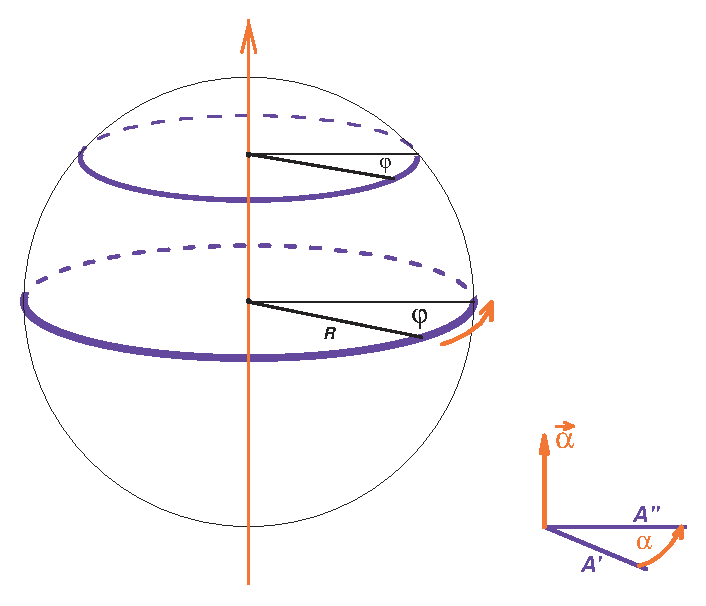
\includegraphics{GP002/GP002F08.eps}}
 \put( 180, 92){\makebox(0,0)[tr]{\parbox{85mm}
     {
     \centerline{\underline{Угловая скорость:}}
      \begin{displaymath}
      \omega=\dot{\varphi}=\frac{d\varphi}{dt}
      \end{displaymath}
     \centerline{\underline{Угловое ускорение:}}
      \begin{displaymath}
      \beta=\dot{\omega}=\ddot{\varphi}=\frac{d\omega}{dt}=\frac{d^2\varphi}{dt^2}
      \end{displaymath}
     }}}
 \put( 175, 0){\makebox(0,0)[br]{\parbox{50mm}
     {
      \centerline{Угол как вектор:}
      \begin{displaymath}
      \vec{\alpha}=\alpha\cdot\frac
          {\left[\vec{A'}\times\vec{A''}\right]}
          {\left|\left[\vec{A'}\times\vec{A''}\right]\right|}
      \end{displaymath}
     }}}
  \end{picture}\\
  \caption{\sf\Large Вращательное движение.}
   \label{fig:rot_move}
\end{figure}

  {\bf Вращение --} все точки тела описывают окружности с центрами на {\sl оси вращения} (Рис.~\ref{fig:rot_move}):

Связь линейной и угловой скорости:

      \begin{displaymath}
      V=\lim_{\Delta t\rightarrow0}\frac{\Delta S}{\Delta t}=\frac{d(R\cdot\varphi)}{dt}=
      \omega R;\;\;\;\;\;\;\;\vec{V}=\left[\vec{\omega}\times\vec{R}\right]
      \end{displaymath}
%\newpage

\underline{\bf Линейные и аксиальные векторы}\\

Линейные (истинные) векторы -- те, что связаны с поступательным движением или направлением в пространстве:

 \begin{displaymath}
 \vec{X}, \vec{Y}, \vec{Z}, \vec{V}, \vec{R}, \vec{a}, \vec{F},
 \end{displaymath}

Аксиальные векторы -- те, что связаны с вращением:

 \begin{displaymath}
 \vec{\varphi}, \vec{\alpha}, \vec{\beta}, \vec{L}, \vec{M}
 \end{displaymath}

Они отличаются своими свойствами симметрии: при зеркальном отра\-жении (то есть, при замене $X \rightarrow -X$) линейные векторы меняют знак, а аксиальные - не меняют (Рис.~\ref{fig:lin_axial_vecs}).

\begin{figure}[htp]
 \setlength{\unitlength}{1mm}
  \begin{picture}(180,150)(0,0)
  %\put(0,0){\framebox(180,150)[b]{}}
   \put(15,0){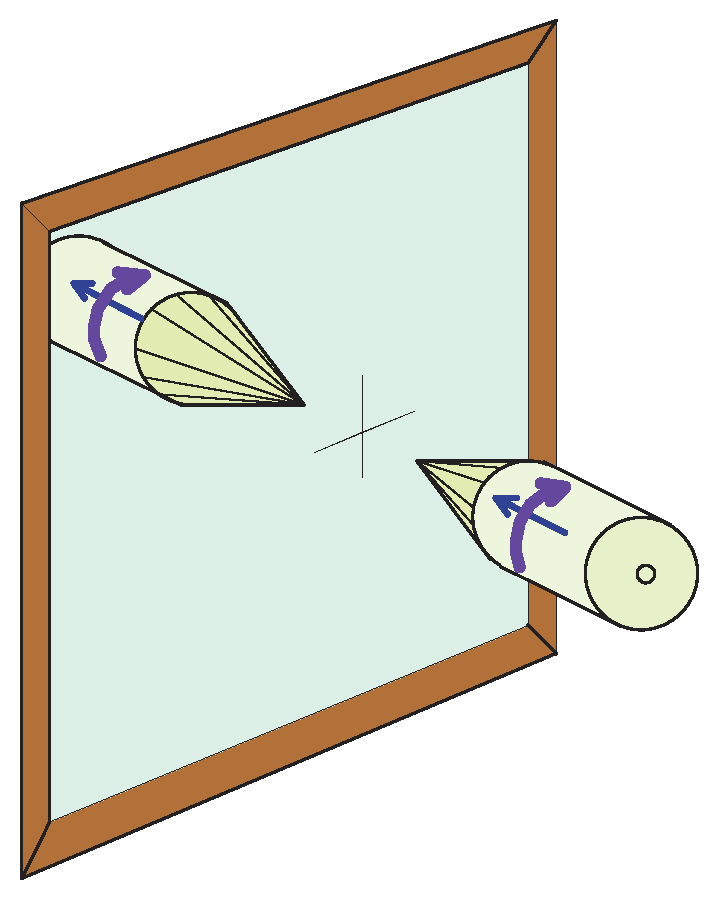
\includegraphics{GP002/GP002F09.eps}}
   \put(48, 105){\makebox(0,0)[c]{\color{blue}\Huge\bf $\vec{\omega}_2$}}
   \put(48, 70){\makebox(0,0)[c]{\color{red}\Huge\bf $\vec{V}_2$}}
   \put(120, 70){\makebox(0,0)[c]{\color{blue}\Huge\bf $\vec{\omega}_1$}}
   \put(120, 35){\makebox(0,0)[c]{\color{red}\Huge\bf $\vec{V}_1$}}
   \put(150,110){\makebox(0,0)[c]{\color{red}\Huge\bf $\vec{V}_2 = -\vec{V}_1$}}
   \put(150, 90){\makebox(0,0)[c]{\color{blue}\Huge\bf $\vec{\omega}_2 = +\vec{\omega}_1$}}
  \end{picture}\\[1mm]
  \caption{\sf\Large Отзеркаливание линейных и аксиальных векторов.}
   \label{fig:lin_axial_vecs}
\end{figure}
  
\newpage
\begin{flushright}
{\color{green}\LARGE\sl ШПАРГАЛКА}
\end{flushright}

\underline{\bf Связь декартовых и сферических координат}

Показана на Рис.~\ref{fig:dec_vs_sphe}.

 \begin{displaymath}
 \left\{\vec{x}, \vec{y}, \vec{z}\right\}
 \;\;\;\leftrightarrow \;\;\;
 \left\{\vec{r}, \vec{\theta}, \vec{\varphi}\right\}
 \end{displaymath}

\begin{figure}[ht]
 \setlength{\unitlength}{1mm}
  \begin{picture}(160,120)(0,0)
  %\put(0,0){\framebox(180,130)[b]{}}
   \put(25,0){\includegraphics{GP002/GP002F10.eps}}
  \end{picture}\\[1mm]
  \caption{\sf\Large Связь декартовых и сферических координат.}
   \label{fig:dec_vs_sphe}
\end{figure}
 
 \begin{displaymath}
 \begin{array}{ccccc}
 0&\leq&r&&\\
 0&\leq&\theta&\leq&\pi\\
 0&\leq&\varphi&\leq&2\pi
 \end{array}
 \end{displaymath}

 \begin{displaymath}
 \left\{
 \begin{array}{ccl}
 x&=&r\sin\theta\cos\varphi\\
 y&=&r\sin\theta\sin\varphi\\
 z&=&r\cos\theta
 \end{array}
 \right\}\;\;\;
 \leftrightarrow\;\;\;
 \left\{
 \begin{array}{ccl}
 r&=&\sqrt{x^2+y^2+z^2}\\
 \theta&=&\arccos\left(z/r\right)\\
 \varphi&=&\arctan\left(y/x\right)
 \end{array}
 \right\}
 \end{displaymath}

 \begin{displaymath}
dx\cdot dy\cdot dz\;\;=\;\;dV\;\;=\;\;r^2\cdot dr\cdot\sin\theta\cdot d\theta\cdot d\varphi
 \end{displaymath}

%\newpage
\begin{flushright}
{\color{green}\LARGE\sl ШПАРГАЛКА}
\end{flushright}
\centerline{\huge\underline{Правила векторной алгебры}}
\begin{itemize}
\item длина вектора (модуль):
 \begin{displaymath}
 |\vec{A}| = \sqrt{A_x^2+A_y^2+A_z^2}
 \end{displaymath}
\item сложение (вычитание):
 \begin{displaymath}
 \vec{C} = \vec{A} \pm \vec{B}\;\;\;\Leftrightarrow\;\;\;
 \left\{\begin{array}{cc}C_x &= A_x\pm B_x\\
                         C_y &= A_y\pm B_y\\
                         C_z &= A_z\pm B_z\end{array}\right.
 \end{displaymath}
\item умножение на число (масштабирование):
 \begin{displaymath}
 \vec{C} = k\cdot\vec{A} \;\;\;\Leftrightarrow\;\;\;
 \left\{\begin{array}{cc}C_x &= k\cdot A_x\\
                         C_y &= k\cdot A_y\\
                         C_z &= k\cdot A_z\end{array}\right.
 \end{displaymath}
\item дифференцирование:
 \begin{displaymath}
 \vec{C} = \frac{\vec{dA}}{dt} \;\;\;\Leftrightarrow\;\;\;
 \left\{\begin{array}{cc}C_x &= {dA_x}/{dt}\\
                         C_y &= {dA_y}/{dt}\\
                         C_z &= {dA_z}/{dt}\end{array}\right.
 \end{displaymath}
\item скалярное перемножение двух векторов:
 \begin{displaymath}
 C = \left(\vec{A},\vec{B}\right) = \vec{A}\cdot\vec{B}\;\;\;\Leftrightarrow\;\;\;
 C = A_x\cdot B_x + A_y\cdot B_y + A_z\cdot B_z =|A|\cdot|B|\cdot \cos\theta
\end{displaymath}
\item векторное перемножение двух векторов:
 \begin{displaymath}
 \vec{C} = \left[\vec{A},\vec{B}\right] = \vec{A}\times\vec{B}\;\;\;\Leftrightarrow\;\;\;
 \left\{\begin{array}{cc}C_x &= A_y\cdot B_z - A_z\cdot B_y\\
                         C_y &= A_z\cdot B_x - A_x\cdot B_z\\
                         C_z &= A_x\cdot B_y - A_y\cdot B_z\end{array}\right.
 \end{displaymath}
 \begin{displaymath}
  |C|=|A|\cdot|B|\cdot\sin\theta;\;\;\;\; \vec{C}\perp\vec{A};\;\;\;\vec{C}\perp\vec{B}
\end{displaymath}
\end{itemize}

